%%
%%  Department of Electrical, Electronic and Computer Engineering.
%%  EPR400/2 Final Report - Section 2.
%%  Copyright (C) 2011-2018 University of Pretoria.
%%



\section{Approach}

The design for the system, as explained in the previous section should contain two main designs, handwriting recognition and communication.

\subsection{Design alternatives}

The data input device to be used to input data onto the device’s touchscreen could either be a light pen or a mouse. The trade-off associated with the choice for the device was that of portability against the degree of detail of the drawing painted on the touchscreen interface by the input device. Another trade-off considered was that of pressure sensitivities on the touchscreen which would gradually damage the touch screen’s display against the degree of detail that would be provided by the input device. 

The Human-Machine Interface functional block could be designed for by comparing the different touchscreen devices available. The available choices were capacitive touchscreens and resistive touchscreens. A trade-off for the touchscreen device to be chosen was that of sensing pen or data input gestures using the chosen data input technique but filtering out input that was not from the data input device like a user’s palm interfering with the drawing while the user was holding the device. 

The device’s control unit block could be designed for using either a micro-controller or a development board. A micro-controller had an advantage of being small. A development board had an advantage of minimizing the overall device’s wiring. If a micro-controller were to be used, a PCB would be required to integrate it with the touchscreen and the communication module to be used. The micro-controller would also need to be integrated with an external microprocessor as well as an external memory module for saving the shopping list data and I/O pins for external serial interface. This would result in a lot of wires in the system that would affect debugging time if mistakes were made. On the other hand, development boards have the microcontroller, the microprocessor, sometimes communication modules, a memory module slot and just about enough I/O pins all on the same lightweight board. Development boards are also programmable using high level programming languages like C++ and Python, making them easier to simulate on PCs.

The handwriting system process is shown in the diagram on the next page.\\\\
The Recognition Algorithm could be designed and implemented using Neural Networks or Hidden Markov Models. An advantage of the neural networks approach was that with increased training data, unseen patterns of line handwriting inputs could be accurately recognized. An advantage of Hidden Markov Models was that the probability of characters being next to each other is considered to estimate patterns with predefined data sets, producing words which are in the dictionary.
\newpage
\begin{figure}[h]
	\centering
	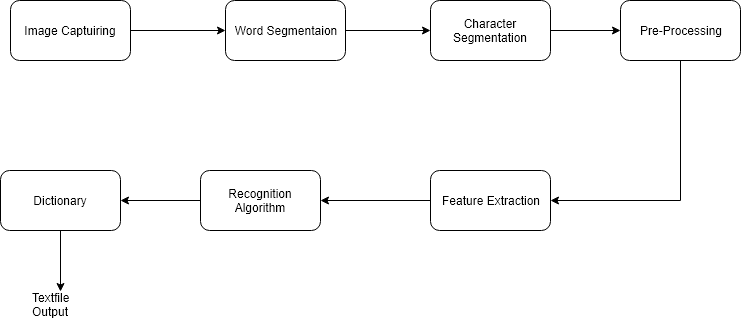
\includegraphics[scale=0.5]{2}
	\caption{Basic Flow diagram showing the modules associated with the handwriting recognition process}
\end{figure}
A diagram of how the general communication is achieved for the device is shown below.
\begin{figure}[h]
	\centering
	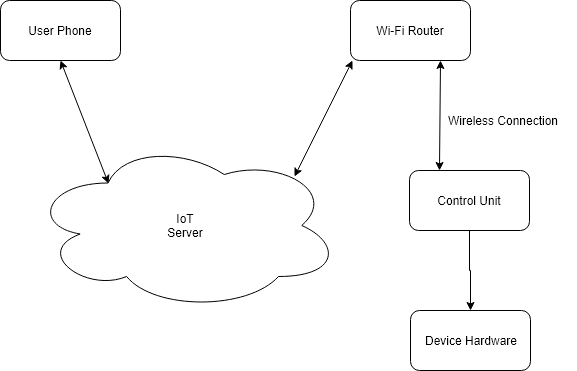
\includegraphics[scale=0.5]{3}
	\caption{General communication system for the device}
\end{figure}

The communication system of the device could be designed and implemented using either GSM communication or Wi-Fi communication. An advantage of GSM is that high speed data transmission is possible. Also, with enough money to cater for roaming costs, data could be transmitted between two devices situated anywhere in the world. An advantage of Wi-Fi is that the network is secure is broadcast data signals can be transmitted to the other device if they have the correct pre-shared key. 

The mobile application to access the shopping list can either be the phone’s SMS system, the phone’s email system or a customized application. An advantage of the SMS system as well as the e-mail system is that it prints the text as it is from the text document from the shopping list device and the. An advantage of the customized application is that it presents the shopping in a more customer-focussed user interface. A button only has to be pressed and the user can access their list.

\subsection{Preferred solution}

A touch pen (stylus) was chosen as the design choice for the input device to be used. This was because a pen more accurately defined a real-world handwriting drawing since in the real-world people use pens and pencils to write. Additionally, a pen is portable and wireless while a Bluetooth connection first is needed for a wireless mouse and the shapes drawn by mice do not accurately model human handwriting styles. An important trade-off when eventually getting the off-the-shelf stylus pen was the pen size against the precision. Bigger stylus pens can be sensed more easily by a touchscreen device, but the drawings produced by them are not precise enough to model real-life handwriting. An optimum size of the pen was supposed to be chosen for portability purposes and reasonable tip size.

A capacitive touchscreen was used as the HMI of the system because it is less susceptible to scratches and permanent damage when a light pen is gently pressed onto the screen compared to resistive screens which require more rigorous pressing for pen drawing detection thus causing the screen to be easily damaged. The trade-off associated with the screen is that of the requirement that it should provide enough visible space for comfortable handwriting input while being small-scale enough to be integrable to the rest of the hardware and keeping the whole device lightweight.

A development board was used for the control unit of the shopping list device. It was chosen because it reduced wiring as explained before and it could easily be simulated on a PC. The development board of choice would have to run an Operating System that also runs on PCs. A trade-off associated with using a development board was finding the optimal price of the device which contained most of the hardware for the desired embedded circuit so that programming the hardware was the most complex part to be done on the control unit. The choices of development boards available to use for the device will vary from Raspberry Pi, to Odroid and Adafruit boards.

A neural network approach was used because the accuracy of the recognition process could be improved as more patterns were input into the system and the algorithm was trained and learned from previous results. A trade-off of the neural network approach was sacrificing accuracy for conversion time. An optimal number of hidden layers was calculated and used so that conversion time could be less than or equal to 1 second as specified in section 3 of the document while the accuracy could be 80% or more. The algorithm was programmed using the Python programming language.

Wi-Fi communication was used instead of GSM. This was because GSM has recurring costs associated with the service provider used and reloading the service requires removing the SIM card from the GSM module, recharging it on a cell-phone and inserting it back onto the module. The device to be developed will be permanently enclosed except for its charging system so this interferes with this condition. Alternatively, recharging is done by complex programming. On the contrary, reloading the Internet service for Wi-Fi is done on the router and no hardware on the shopping list device is interfered with. A trade-off associated with Wi-Fi communication is that of power consumption against transmission speed. [1]. Since the desire is to transmit data over a long range, an optimum speed should be designed for where the device does not run out of power whole in the process of transmitting the shopping list data.

The e-mail system application was used because this is an everyday application that most cell phone users are familiar with. A customized application was to be additionally programmed using Android Studio instead of Qt due to its mobile-focussed platform for mobile application development.

\newpage

%% End of File.

